شبکه عصبی پیچشی تکه‌ای\LTRfootnote{Piecewise Convolutional Neural Network(PCNN)} در ابتدا در سال ۲۰۱۵ توسط ژنگ و همکاران در کنفرانس \lr{ACL} ارائه شد
\cite{zeng-etal-2015-distant}. این شبکه با هدف استخراج روابط بین دو موجودیت در متن ارائه شد. در سال‌های بعد
هم «استخراج رابطه بین موجودیت‌ها» هدف بیشتر  پژوهش‌هایی بود که از این شبکه عصبی استفاده کردند.

با توجه تنیدگی شبکه عصبی پیچشی تکه‌ای و استخراج رابطه نیاز است تا توضیحاتی در رابطه با
شیوه استخراج رابطه بین موجودیت‌ها در متن داده شود.
در استخراج رابطه موجودیت‌ها از روی جمله تلاش می‌شود با داشتن موجودیت‌ها و متن جمله،
رابطه‌ای که جمله بین آن‌ موجودیت‌ها بیان می‌کند، استخراج شود. برای روشن شدن مطلب جمله «حافظ در شیراز درگذشت.» را
در نظر بگیرید.
این جمله شامل دو موجودیت «حافظ» و «شیراز» بوده و رابطه بیان شده توسط این جمله برای این دو موجودیت «محل فوت» است.
هدف این پژوهش‌ها نیز استخراج رابطه «محل فوت» از روی متن جمله و موجودیت‌های آن است.

گرچه استخراج رابطه از متن در نگاه اول ساده به نظر می‌رسد اما این پژوهش‌ها با چالش‌هایی نیز مواجهند. در مثال قبلی جمله رابطه «محل فوت» را بین دو موجودیت
«حافظ» و «شیراز» بیان می‌کرد اما جمله «حافظ در شیراز متولد شد» رابطه «محل تولد» را بین دو موجودیت بیان می‌کند.
همان‌طور که می‌بینید با اندکی تغییر در جمله معنای جمله کاملا می‌تواند متفاوت شود و رابطه دیگری را بین موجودیت‌ها بیان کند.

برای فراهم کردن داده‌های آموزشی برای استخراج رابطه در گذشته از روش‌های بانظارت استفاده می‌شد. اما با توجه به سرآیند زیاد این
روش‌ها مینتز در سال ۲۰۰۹ ایده نظارت‌ازراه‌دور را برای جمع‌آوری داده برای وظیفه استخراج رابطه از روی جمله را
مطرح کرد \cite{mintz-etal-2009-distant}. در این ایده از یک پایگاه دانش که شامل موجودیت‌ها و رابطه بین آن‌ها بود
برای جمع‌آوری داده‌های آموزشی از سطح وب استفاده می‌شود. بدین طریق که هر جمله‌ای که شامل هر دو موجودیت بود به عنوان
نمونه‌ای از رابطه‌ی بیان شده بین دو جمله در نظر گرفته می‌شود. البته همان‌طور که مشخص است این ایده ممکن است جملاتی را نیز
که رابطه دیگری را بیان می‌کنند را به عنوان یک نمونه آموزشی برای رابطه مدنظر جمع‌آوری کند، مثلا این ایده هر دو مثال
ارائه شده در بالا را به عنوان «محل فوت» یا «محل زندگی» در نظر می‌گیرد.
اما از آن جا که حجم داده‌های آموزشی جمع‌آوری شده در این حالت
بسیار زیاد است در مصالحه بین حجم داده برچسب خورده و درستی برچسب‌ها این روش بهتر عمل می‌کند.

حال که زمینه پژوهشی استخراج رابطه از متن بررسی شد، تمرکز خود را روی شبکه عصبی \lr{PCNN} و تلاش‌هایی که برای
بهبود آن انجام شده است می‌دهیم. در ابتدا شیوه عمل شبکه عصبی پیچشی تکه‌ای را مورد بررسی قرار می‌دهیم.

\begin{figure}[h]
    \centering
    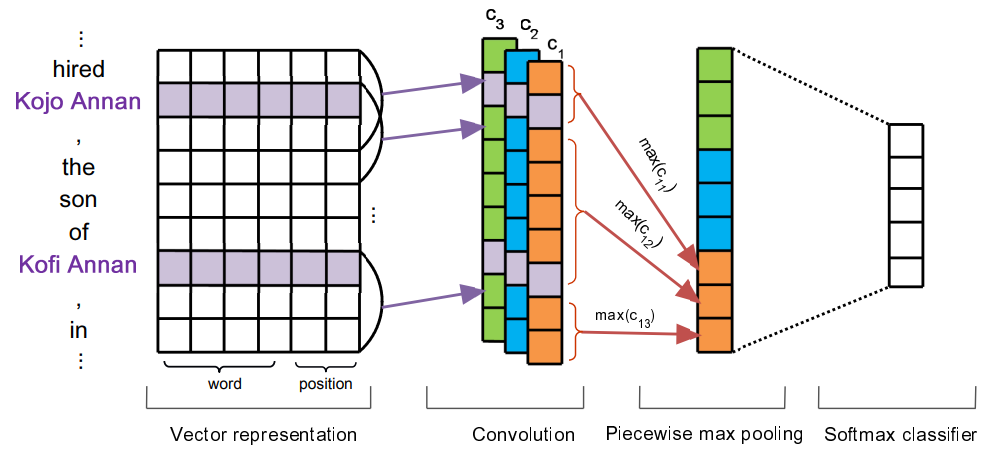
\includegraphics[width=0.8\linewidth]{images/pcnn.png}
    \caption{شبکه عصبی پیچشی تکه‌ای}
    \label{pcnn_architecture}
\end{figure}

در شکل \ref{pcnn_architecture} ساختار شبکه عصبی پیچشی تکه‌ای مشاهده می‌شود. با ورود نمایش برداری کلمات به لایه‌های
کانوولوشنی، این لایه‌ها به صورت سطری روی نمایش برداری پیمایش کرده و ویژگی‌های جمله را استخراج می‌کنند. در ادامه
هر بردار ویژگی استخراج شده توسط لایه کانوولوشنی به سه قسمت تقسیم می‌شود: قسمت قبل از موجودیت اول، قسمت مابین
موجودیت اول و دوم و قسمت بعد از موجودیت دوم. بیشینه هر یک از این قسمت‌ها محاسبه شده و به صورت یک بردار سه‌تایی
در می‌آید. بردار نهایی بازنمایی جمله با ترکیب بردار‌های سه‌تایی متناظر هر یک از لایه‌های کانوولوشنی حاصل می‌شود. در قدم
بعد از این بازنمایی برای کاربرد مدنظر استفاده می‌شود. به عبارتی شبکه \lr{PCNN} یک شبکه کدگذار است که با دریافت یک بازنمایی
با طول متغیر آن را به یک بازنمایی با طول ثابت نگاشت می‌کند. استخراج ویژگی‌های خوب به همراه ارائه بردار با طول ثابت
برای بازنمایی‌های با طول متغیر باعث محبوبیت شبکه‌های عصبی تکه‌ای شده است.

برای بهبود این شبکه‌های عصبی راهکار‌های مختلفی ارائه شده است. یکی از راهکار‌ها مدل ارائه شده توسط پنگ و همکاران
\cite{dilated} است. آن‌ها پیشنهاد کردند برای آن‌ که شبکه عصبی \lr{PCNN} بتواند وابستگی‌های با فاصله زیاد را در جمله
بهتر بازنمایی کند، به جای استفاده از کانوولوشن‌های پیوسته از کانوولوشن‌های دراز\LTRfootnote{dilated} استفاده شود. این لایه‌های
کانوولوشن به جای آن که خروجی را از روی بردار‌های نزدیک به هم محاسبه کند از بردار‌های با فاصله مکانی مشخص
استفاده می‌کند.

شیوه دیگری که برای بهبود این شبکه‌ها استفاده شده است، ترکیب شبکه‌های عصبی بازگشتی با این شبکه‌هاست. این ایده اولین
بار توسط یان و هو \cite{lstm-pcnn} ارائه شد. بازنمایی ارائه شده توسط شبکه عصبی \lr{PCNN} برای هر بخش بازنمایی
مستقلی را ارائه می‌دهد، بنابراین آن‌ها قصد داشتند با عبور بازنمایی تولید شده از
شبکه عصبی حافظه کوتاه‌مدت بلند\LTRfootnote{Long short-term memory} از این استقلال بکاهند.

اما بیشتر پژوهش‌ها تلاش کرده‌اند عملکرد شبکه‌های پیچشی تکه‌ای را با ارائه بازنمایی بهتر از ورودی‌ها بهبود
ببخشند. اکثر این پژوهش‌ها تلاش دارند که با وزن‌دهی به اجزای مهم در ورودی بازنمایی بهتری را با استفاده
از شبکه‌های پیچشی تکه‌ای تولید کنند \cite{nguyen-vietnamese}, \cite{agpcnn-xingya},
\cite{RCPNN-haihong}, \cite{Rusnachenko-opinion} \cite{Li2022}, \cite{gated}. تحقیقات دیگر ایده‌های دیگری برای بهبود عملکرد این شبکه
عصبی پیشنهاد کردند. برای مثلا سانگها نام\LTRfootnote{Sangha Nam} و همکاران \cite{nam-etal-2018-distant} تلاش کردند
بازنمایی بهتری را در ورودی شبکه‌های عصبی پیچشی تکه‌ای برای کلماتی که چندمعنا دارند ارائه دهند. روش پیشنهادی
آن‌ها برای این کار استفاده از یک ماژول ابهام‌زدایی از کلمات بود. در پژوهش دیگری که در سال ۲۰۱۹ انجام شد
تلاش شد با استفاده سلسله‌مراتبی از مدل \lr{PCNN} نتیجه بهتری کسب شود \cite{diyah-adpcnn}.

بعضی دیگر نیز ایده بیان شده توسط شبکه‌های پیچشی تکه‌ای را به شکل دیگری استفاده کرده‌اند. در شبکه
عصبی پیچشی تکه‌ای ابتدا کانوولوشن روی ورودی اعمال شده و سپس خروجی به چند تکه تقسیم می‌شود
اما در مقاله ارائه شده توسط لیو\LTRfootnote{Liu} و همکاران پیشنهاد شد ابتدا ورودی تکه‌تکه شود
و سپس عمل کانوولوشن روی هر قسمت انجام شود \cite{bert}.

به عنوان سخن آخر می‌خواهیم به کاربرد‌های شبکه عصبی \lr{PCNN} در سایز حوزه‌ها اشاره ‌کنیم.
برای این کار می‌توان از پژوهش‌های انجام شده توسط دو\LTRfootnote{Du} و ژنگ\LTRfootnote{Zhang} نام‌ برد.
هر دو این پژوهش‌ها تلاش کرده‌اند با استفاده از شبکه‌های عصبی پیچشی تکه‌ای به نتایج بهتری در حوزه
تحلیل منظور\LTRfootnote{sentiment analysis} انجام دهد. دو از شبکه \lr{PCNN} به عنوان یک کدگذار
استفاده می‌کند و برای افزایش تعداد نمونه‌های آموزشی از شبکه‌های مولد تقابلی\LTRfootnote{Generative Adversarial Network}
بهره می‌گیرد \cite{sentiment-du}. ژنگ نیز مشابه دو به منظور کدگذاری جملات ورودی از شبکه‌های عصبی پیچشی تکه‌ای استفاده
می‌کند \cite{Zhang2018SentimentCB}.

در بخش‌های بعدی با جزئیات برخی از کار‌هایی که در زمینه شبکه‌های عصبی پیچشی تکه‌ای شاخص هستند، را بررسی خواهیم کرد.
در انتها نیز خلاصه‌ای از مطالب ارائه شده و لیست مراجع استفاده شده را خواهیم داشت.